\documentclass[border=12pt,12pt]{standalone}
\usepackage[T1]{fontenc}
\usepackage{lmodern}
\usepackage{xcolor}
\usepackage{tikz}
\usetikzlibrary{shapes.geometric,shapes.multipart,arrows.meta,positioning,fit,calc}
\setlength{\textwidth}{16cm}
\setlength{\linewidth}{16cm}
\tikzset{
  umlclass/.style={rectangle split, rectangle split parts=3, draw, fill=white,
    font=\scriptsize, text width=5.2cm, align=left, inner sep=3pt},
  usecase/.style={ellipse, draw, fill=white, font=\footnotesize, minimum width=3.4cm,
    minimum height=0.8cm, align=center},
  act/.style={rectangle, rounded corners=6pt, draw, fill=white, font=\footnotesize,
    minimum width=4.2cm, minimum height=0.7cm, align=center},
  dec/.style={diamond, draw, fill=white, aspect=2.2, font=\scriptsize, inner sep=1pt, align=center},
  flow/.style={-{Stealth[length=2.2mm]}, thick},
  assoc/.style={-, thick},
  compo/.style={{Diamond[fill=black,length=3mm,width=2mm]}-, thick},
  aggr/.style={{Diamond[open,length=3mm,width=2mm]}-, thick},
  depend/.style={-{Stealth[length=2mm]}, dashed, thick},
  msg/.style={-{Stealth[length=2mm]}, thick},
  ret/.style={-{Stealth[length=2mm]}, dashed},
}
\newcommand{\actor}[2]{% #1 node name, #2 label
  \begin{scope}[shift={(#1)}]
    \draw[thick] (0,0.55) circle (0.18);
    \draw[thick] (0,0.37) -- (0,-0.1);
    \draw[thick] (-0.3,0.2) -- (0.3,0.2);
    \draw[thick] (0,-0.1) -- (-0.22,-0.5);
    \draw[thick] (0,-0.1) -- (0.22,-0.5);
    \node[font=\footnotesize, below] at (0,-0.5) {#2};
  \end{scope}}


\begin{document}
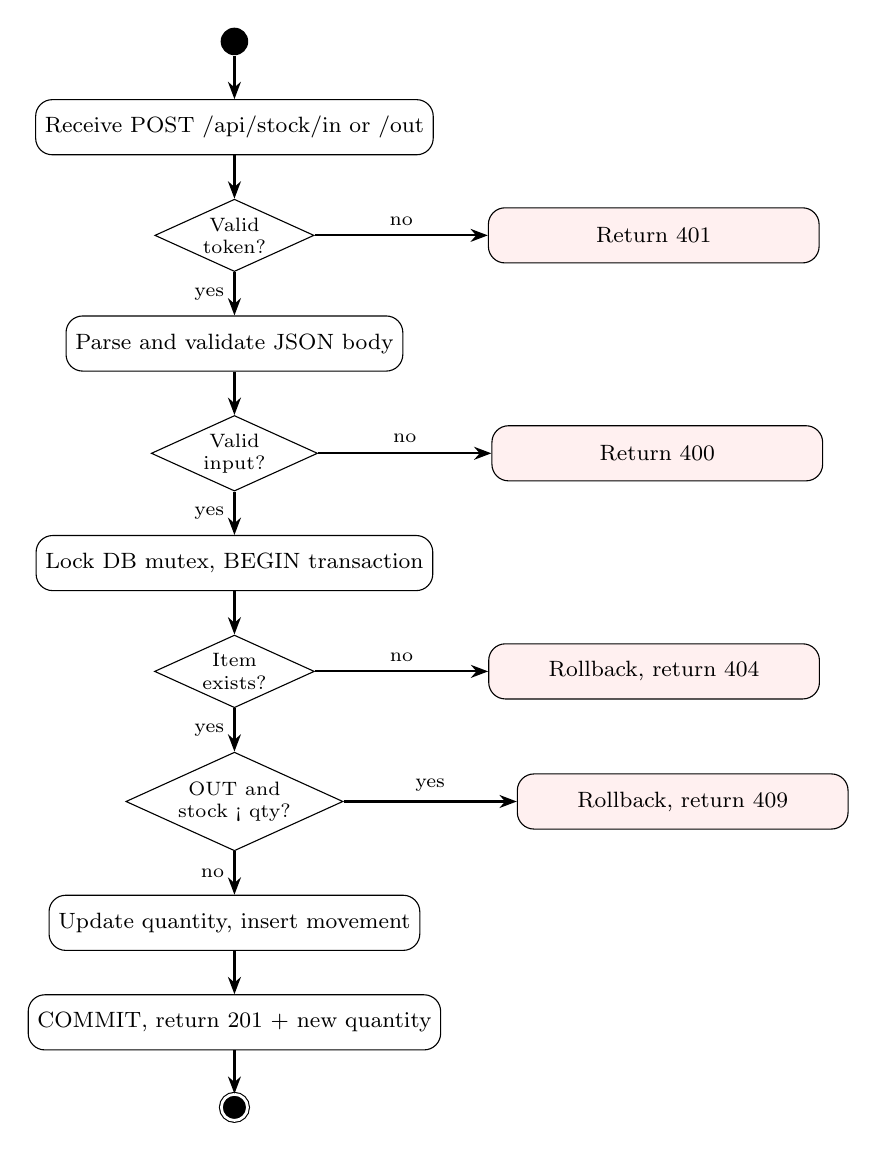
\begin{tikzpicture}[node distance=0.55cm]
  \node[circle, fill=black, minimum size=0.35cm] (start) {};
  \node[act, below=of start] (a1) {Receive POST /api/stock/in or /out};
  \node[dec, below=of a1] (d1) {Valid\\token?};
  \node[act, below=of d1] (a2) {Parse and validate JSON body};
  \node[dec, below=of a2] (d2) {Valid\\input?};
  \node[act, below=of d2] (a3) {Lock DB mutex, BEGIN transaction};
  \node[dec, below=of a3] (d3) {Item\\exists?};
  \node[dec, below=of d3] (d4) {OUT and\\stock < qty?};
  \node[act, below=of d4] (a4) {Update quantity, insert movement};
  \node[act, below=of a4] (a5) {COMMIT, return 201 + new quantity};
  \node[circle, draw, double, double distance=1pt, fill=black, minimum size=0.3cm, below=of a5] (end) {};
  \node[act, right=2.2cm of d1, fill=red!6] (e1) {Return 401};
  \node[act, right=2.2cm of d2, fill=red!6] (e2) {Return 400};
  \node[act, right=2.2cm of d3, fill=red!6] (e3) {Rollback, return 404};
  \node[act, right=2.2cm of d4, fill=red!6] (e4) {Rollback, return 409};
  \draw[flow] (start) -- (a1);
  \draw[flow] (a1) -- (d1);
  \draw[flow] (d1) -- node[left, font=\scriptsize]{yes} (a2);
  \draw[flow] (a2) -- (d2);
  \draw[flow] (d2) -- node[left, font=\scriptsize]{yes} (a3);
  \draw[flow] (a3) -- (d3);
  \draw[flow] (d3) -- node[left, font=\scriptsize]{yes} (d4);
  \draw[flow] (d4) -- node[left, font=\scriptsize]{no} (a4);
  \draw[flow] (a4) -- (a5);
  \draw[flow] (a5) -- (end);
  \draw[flow] (d1) -- node[above, font=\scriptsize]{no} (e1);
  \draw[flow] (d2) -- node[above, font=\scriptsize]{no} (e2);
  \draw[flow] (d3) -- node[above, font=\scriptsize]{no} (e3);
  \draw[flow] (d4) -- node[above, font=\scriptsize]{yes} (e4);
\end{tikzpicture}
\end{document}
